\documentclass{article}

% content/resources/templates/preamble.tex
\usepackage[margin=0.6in]{geometry}
\author{Milav Dabgar}
\usepackage{amsmath,amssymb,amsthm}
\usepackage{booktabs}
\usepackage{multirow}
\usepackage{xcolor}
\usepackage{tcolorbox}
\tcbuselibrary{breakable,skins}
\usepackage[colorlinks=true,linkcolor=blue]{hyperref}
\usepackage{titlesec}
\usepackage{enumitem}
\usepackage{tikz}
\usepackage{pgfplots}
\usepackage{circuitikz}
\usepackage[version=4]{mhchem}
\usepackage{longtable}
\usepackage{array}
\usepackage{float}
\usepackage{caption}
\usepackage{listings}

\lstset{
  basicstyle=\small\ttfamily,
  breaklines=true,
  breakatwhitespace=false,
  postbreak=\mbox{\textcolor{red}{$\hookrightarrow$}\space},
  float=false,
  numbers=left,
  numberstyle=\tiny\color{gray},
  numbersep=10pt,
  xleftmargin=2em,
  keywordstyle=\color{blue},
  commentstyle=\color{green!60!black},
  stringstyle=\color{purple},
  backgroundcolor=\color{gray!5},
  showstringspaces=false,
  tabsize=2,
  captionpos=b,
  keepspaces=true,
  columns=flexible
}

\pgfplotsset{compat=1.18}
\usetikzlibrary{shapes,arrows,positioning,calc,patterns,decorations.pathmorphing,decorations.markings,arrows.meta}

% Color scheme
\definecolor{headcolor}{RGB}{0,102,204}
\definecolor{keycolor}{RGB}{220,20,60}
\definecolor{solutioncolor}{RGB}{34,139,34}
\definecolor{mnemoniccolor}{RGB}{148,0,211}
\definecolor{codecolor}{RGB}{0,0,100}

% Spacing
\setlength{\parskip}{3pt}
\setlist[itemize]{nosep}
\setlist[enumerate]{nosep}

% Title formatting
\titleformat{\section}{\Large\bfseries\color{headcolor}}{\thesection}{1em}{}
\titleformat{\subsection}{\large\bfseries\color{headcolor}}{\thesubsection}{1em}{}

% Pandoc tightlist compatibility
\providecommand{\tightlist}{%
  \setlength{\itemsep}{0pt}\setlength{\parskip}{0pt}}

% Pandoc longtable compatibility
\newcounter{none}
\def\thenone{}


% content/resources/templates/english-boxes.tex

% Custom environments
\newtcolorbox{solutionbox}{
 breakable,
 enhanced,
 colback=solutioncolor!5!white,
 colframe=solutioncolor!75!black,
 fonttitle=\bfseries,
 title=Solution
}

\newtcolorbox{solutionboxnobreak}{
 colback=solutioncolor!5!white,
 colframe=solutioncolor!75!black,
 fonttitle=\bfseries,
 title=Solution
}

\newtcolorbox{keyformula}{
 breakable,
 enhanced,
 colback=keycolor!5!white,
 colframe=keycolor!75!black,
 fonttitle=\bfseries,
 title=Key Formula
}

\newtcolorbox{mnemonicboxenv}{
 breakable,
 enhanced,
 colback=mnemoniccolor!5!white,
 colframe=mnemoniccolor!75!black,
 fonttitle=\bfseries,
 title=Mnemonic
}

\newcommand{\mnemonicbox}[1]{%
  \begin{mnemonicboxenv}
    #1
  \end{mnemonicboxenv}
}


% Custom commands for GTU solutions
% This file defines semantic commands for consistent formatting

% Question command with automatic formatting
\newcommand{\question}[2]{%
  \section*{Question #1}%
  \textbf{#2}%
}

% OR question variant
\newcommand{\questionor}[2]{%
  \section*{Question #1 OR}%
  \textbf{#2}%
}

% Proper table environment with caption
\newenvironment{answertable}[1]{%
  \begin{table}[htbp]
  \centering
  \caption{#1}
}{%
  \end{table}
}

% Proper figure environment for diagrams
\newenvironment{answerdiagram}[1]{%
  \begin{figure}[htbp]
  \centering
  \caption{#1}
}{%
  \end{figure}
}

% Semantic markup for key terms
\newcommand{\keyword}[1]{\textbf{#1}}
\newcommand{\code}[1]{\texttt{#1}}
\newcommand{\classname}[1]{\texttt{#1}}
\newcommand{\methodname}[1]{\texttt{#1}}

% Proper quotation marks
\newcommand{\mnemonic}[1]{``#1''}

\usetikzlibrary{mindmap,trees}

\title{Microprocessor and Microcontroller (4341101) - Winter 2023 Solution}
\date{December 15, 2023}

\begin{document}
\maketitle

\questionmarks{1}{a}{3}
\textbf{Compare RISC and CISC.}

\begin{solutionbox}
\textbf{Answer}:

\begin{center}
\captionof{table}{RISC vs CISC}
\begin{tabulary}{\linewidth}{|l|J|J|}
\hline
\textbf{Feature} & \textbf{RISC} & \textbf{CISC} \\ \hline
\textbf{Instructions} & Simple, fixed-length & Complex, variable-length \\ \hline
\textbf{Execution} & Single cycle & Multiple cycles \\ \hline
\textbf{Addressing modes} & Few & Many \\ \hline
\textbf{Registers} & Many & Few \\ \hline
\textbf{Design focus} & Hardware simplicity & Code density \\ \hline
\end{tabulary}
\end{center}
\end{solutionbox}
\begin{mnemonicbox}
``RISCs Complete Instructions Simply''
\end{mnemonicbox}

\questionmarks{1}{b}{4}
\textbf{Compare Von-Neumann and Harvard architecture.}

\begin{solutionbox}
\textbf{Answer}:

\begin{center}
\captionof{table}{Von-Neumann vs Harvard}
\begin{tabulary}{\linewidth}{|l|J|J|}
\hline
\textbf{Feature} & \textbf{Von-Neumann} & \textbf{Harvard} \\ \hline
\textbf{Memory} & Single shared memory & Separate program \& data memory \\ \hline
\textbf{Bus} & Single bus for data \& instructions & Separate buses \\ \hline
\textbf{Speed} & Slower (memory bottleneck) & Faster (parallel access) \\ \hline
\textbf{Complexity} & Simpler design & More complex \\ \hline
\textbf{Applications} & General computing & Real-time systems \\ \hline
\end{tabulary}
\end{center}

\textbf{Diagram:}

\begin{center}
\begin{tikzpicture}[node distance=2cm, auto]
    % Von Neumann
    \node (vn) {\textbf{Von-Neumann}};
    \node [gtu block, below of=vn, node distance=1cm] (cpu1) {CPU};
    \node [gtu block, right of=cpu1, node distance=3.5cm] (mem1) {Memory\\(Data + Inst)};
    \draw [gtu arrow, <->] (cpu1) -- (mem1);
    
    % Harvard
    \node [right of=vn, node distance=7cm] (hv) {\textbf{Harvard}};
    \node [gtu block, below of=hv, node distance=1cm] (cpu2) {CPU};
    \node [gtu block, above right of=cpu2, node distance=3cm] (pmem) {Program\\Memory};
    \node [gtu block, below right of=cpu2, node distance=3cm] (dmem) {Data\\Memory};
    
    \draw [gtu arrow, ->] (pmem) -| (cpu2);
    \draw [gtu arrow, <->] (cpu2) |- (dmem);
\end{tikzpicture}
\end{center}
\end{solutionbox}
\begin{mnemonicbox}
``Harvard Has Separate Spaces''
\end{mnemonicbox}

\questionmarks{1}{c}{7}
\textbf{Explain: 8085 Instruction Format, Control Unit, Machine Cycle, ALU}

\begin{solutionbox}
\textbf{Answer}:

\textbf{1. Instruction Format:}
\begin{center}
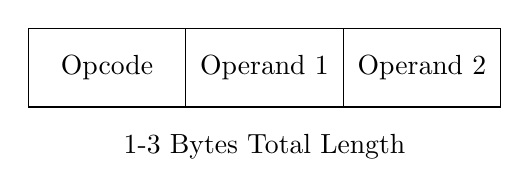
\begin{tikzpicture}
    \draw (0,0) rectangle (2,1) node[pos=0.5] {Opcode};
    \draw (2,0) rectangle (4,1) node[pos=0.5] {Operand 1};
    \draw (4,0) rectangle (6,1) node[pos=0.5] {Operand 2};
    \node at (3, -0.5) {1-3 Bytes Total Length};
\end{tikzpicture}
\end{center}
Contains opcode (3-8 bits) and 0-2 operands.

\textbf{2. Explanations:}
\begin{center}
\captionof{table}{Components}
\begin{tabulary}{\linewidth}{|l|J|}
\hline
\textbf{Component} & \textbf{Function} \\ \hline
\textbf{Instruction Format} & 1-3 byte structure with opcode and operands \\ \hline
\textbf{Control Unit} & Fetches, decodes instructions; generates signals \\ \hline
\textbf{Machine Cycle} & Basic operation cycle (T-states) \\ \hline
\textbf{ALU} & Performs arithmetic and logical operations \\ \hline
\end{tabulary}
\end{center}

\textbf{3. Diagram:}
\begin{center}
\begin{tikzpicture}[node distance=2.5cm, auto]
    \node [gtu block] (cu) {Control Unit\\(Sequencer)};
    \node [gtu block, right of=cu, node distance=3.5cm] (ir) {Instruction\\Register};
    \node [gtu block, below of=cu] (alu) {ALU};
    \node [gtu block, right of=alu, node distance=3.5cm] (reg) {Registers};
    
    \draw [gtu arrow, <-] (cu) -- (ir);
    \draw [gtu arrow, <-] (alu) -- (reg);
    \draw [gtu arrow, ->] (alu) -- (reg);
    
    \node [draw, dashed, fit=(cu) (ir) (alu) (reg), label=above:CPU Core] {};
\end{tikzpicture}
\end{center}
\end{solutionbox}
\begin{mnemonicbox}
``CIMA: Control Interprets, Machine Acts''
\end{mnemonicbox}

\orquestionmarks{1}{c}{7}
\textbf{Compare Microprocessor and Microcontroller.}

\begin{solutionbox}
\textbf{Answer}:

\begin{center}
\captionof{table}{Microprocessor vs Microcontroller}
\begin{tabulary}{\linewidth}{|l|J|J|}
\hline
\textbf{Feature} & \textbf{Microprocessor} & \textbf{Microcontroller} \\ \hline
\textbf{Design} & CPU only & CPU + peripherals \\ \hline
\textbf{Memory} & External & Internal (RAM/ROM) \\ \hline
\textbf{I/O ports} & Limited & Many built-in \\ \hline
\textbf{Cost} & Higher & Lower \\ \hline
\textbf{Applications} & General computing & Embedded systems \\ \hline
\textbf{Power} & Higher & Lower \\ \hline
\textbf{Example} & Intel 8085/8086 & Intel 8051 \\ \hline
\end{tabulary}
\end{center}

\textbf{Diagram:}

\begin{center}
\begin{tikzpicture}[node distance=2cm, auto, scale=0.8, transform shape]
    % Microprocessor
    \node (mp) {\textbf{Microprocessor System}};
    \node [gtu block, below of=mp, node distance=1.5cm] (cpu) {CPU};
    \node [gtu block, left of=cpu, node distance=3cm] (mem) {Memory};
    \node [gtu block, right of=cpu, node distance=3cm] (io) {I/O};
    \draw [gtu arrow, <->] (cpu) -- (mem);
    \draw [gtu arrow, <->] (cpu) -- (io);
    \node [below of=cpu, node distance=1.5cm] {Separate Chips};
    
    % Microcontroller
    \node [right of=mp, node distance=8cm] (mc) {\textbf{Microcontroller}};
    \node [gtu block, below of=mc, node distance=2.5cm, minimum width=6cm, minimum height=4cm] (chip) {};
    \node [at=(chip.north), anchor=north] {Single Chip};
    
    \node [gtu block, below of=mc, node distance=1.5cm] (mcpu) {CPU};
    \node [gtu block, left of=mcpu, node distance=2cm] (mmem) {Memory};
    \node [gtu block, right of=mcpu, node distance=2cm] (mio) {I/O};
    
    \draw [gtu arrow, <->] (mcpu) -- (mmem);
    \draw [gtu arrow, <->] (mcpu) -- (mio);
\end{tikzpicture}
\end{center}
\end{solutionbox}
\begin{mnemonicbox}
``Micro-P Processes, Micro-C Controls''
\end{mnemonicbox}

\questionmarks{2}{a}{3}
\textbf{Explain Instruction Fetching, Decoding and Execution Operation in microprocessor.}

\begin{solutionbox}
\textbf{Answer}:

\begin{center}
\captionof{table}{Operation Phases}
\begin{tabulary}{\linewidth}{|l|J|}
\hline
\textbf{Phase} & \textbf{Operation} \\ \hline
\textbf{Fetching} & CPU gets instruction from memory using PC \\ \hline
\textbf{Decoding} & Determines operation type and operands \\ \hline
\textbf{Execution} & Performs the actual operation \\ \hline
\end{tabulary}
\end{center}

\textbf{Diagram:}
\begin{center}
\begin{tikzpicture}[node distance=3cm, auto]
    \node [gtu block] (fetch) {Fetch};
    \node [gtu block, right of=fetch] (decode) {Decode};
    \node [gtu block, right of=decode] (exec) {Execute};
    
    \draw [gtu arrow] (fetch) -- (decode);
    \draw [gtu arrow] (decode) -- (exec);
    \draw [gtu arrow, ->] (exec.south) -- ++(0,-0.5) -| (fetch.south);
\end{tikzpicture}
\end{center}
\end{solutionbox}
\begin{mnemonicbox}
``FDE: First Get, Then Understand, Finally Do''
\end{mnemonicbox}

\questionmarks{2}{b}{4}
\textbf{Explain Bus Organization of 8085 microprocessor.}

\begin{solutionbox}
\textbf{Answer}:

\begin{center}
\captionof{table}{8085 Buses}
\begin{tabulary}{\linewidth}{|l|l|J|}
\hline
\textbf{Bus Type} & \textbf{Width} & \textbf{Function} \\ \hline
\textbf{Address Bus} & 16-bit & Carries memory addresses (A0-A15) \\ \hline
\textbf{Data Bus} & 8-bit & Transfers data (D0-D7) \\ \hline
\textbf{Control Bus} & Various & Manages data flow (RD, WR, IO/M) \\ \hline
\textbf{Multiplexed} & AD0-AD7 & Lower address bits + data bits \\ \hline
\end{tabulary}
\end{center}

\textbf{Diagram:}
\begin{center}
\begin{tikzpicture}[node distance=3cm, auto]
    \node [gtu block] (8085) {8085\\Microprocessor};
    \node [gtu block, right of=8085, node distance=5cm] (mem) {Memory / I/O};
    
    \draw [->, thick] (8085.60) -- (mem.120) node[midway, above] {Address Bus (16-bit)};
    \draw [<->, thick] (8085.0) -- (mem.180) node[midway, above] {Data Bus (8-bit)};
    \draw [->, dashed] (8085.-60) -- (mem.-120) node[midway, below] {Control Bus};
\end{tikzpicture}
\end{center}
\end{solutionbox}
\begin{mnemonicbox}
``ADC: Address points, Data flows, Control directs''
\end{mnemonicbox}

\questionmarks{2}{c}{7}
\textbf{Describe architecture of 8085 microprocessor with the help of neat diagram.}

\begin{solutionbox}
\textbf{Answer}:

\textbf{Diagram:}
\begin{center}
\begin{tikzpicture}[node distance=2cm, auto, scale=0.8, transform shape]
    % Registers
    \node [gtu block, minimum width=2.5cm] (acc) {Accumulator (8)};
    \node [gtu block, below of=acc] (tmp) {Temp Reg};
    \node [gtu block, below of=tmp] (flag) {Flags (5)};
    \node [gtu block, right of=tmp, node distance=3.5cm] (alu) {ALU (8)};
    
    \draw [gtu arrow, <->] (acc) -- (tmp);
    \draw [gtu arrow] (tmp) -- (alu);
    \draw [gtu arrow] (alu) -- (flag);
    
    % General Registers
    \node [gtu block, right of=alu, node distance=4cm, minimum width=3cm] (regs) {
        B (8) | C (8) \\
        D (8) | E (8) \\
        H (8) | L (8)
    };
    \node [gtu block, below of=regs, node distance=2cm, minimum width=3cm] (sp) {SP (16)};
    \node [gtu block, below of=sp, node distance=1.5cm, minimum width=3cm] (pc) {PC (16)};
    
    % Control
    \node [gtu block, left of=flag, node distance=3.5cm] (ir) {Instruction\\Register};
    \node [gtu block, below of=ir] (dec) {Decoder};
    \node [gtu block, below of=dec] (timing) {Timing \&\\Control};
    
    \draw [gtu arrow] (ir) -- (dec);
    \draw [gtu arrow] (dec) -- (timing);
    
    % Buffers
    \node [gtu block, below of=pc, node distance=2cm] (addr) {Address Buffer};
    \node [gtu block, left of=addr, node distance=3.5cm] (data) {Data/Address Buffer};
    
    % Connections
    \node [draw, dashed, above of=regs, node distance=2cm] (bus) {Internal 8-bit Bus};
    \draw [gtu arrow, <->] (bus) -- (acc);
    \draw [gtu arrow, <->] (bus) -- (regs);
    \draw [gtu arrow, <->] (bus) -- (ir);
    
\end{tikzpicture}
\end{center}

\begin{itemize}
    \item \textbf{ALU}: Performs arithmetic \& logical operations
    \item \textbf{Registers}: Store data temporarily (A, B, C, D, E, H, L)
    \item \textbf{Control Unit}: Fetches \& decodes instructions
    \item \textbf{PC}: Points to next instruction address
    \item \textbf{SP}: Points to top of stack
\end{itemize}
\end{solutionbox}
\begin{mnemonicbox}
``ARCBD: Architecture Registers Control Buses Data''
\end{mnemonicbox}

\orquestionmarks{2}{a}{3}
\textbf{Explain De-multiplexing of Address and Data buses for 8085 Microprocessor.}

\begin{solutionbox}
\textbf{Answer}:

\begin{enumerate}
    \item \textbf{ALE High}: Lower address (A0-A7) appears on AD0-AD7 lines. Latch captures it.
    \item \textbf{ALE Low}: AD0-AD7 lines are used for Data (D0-D7).
\end{enumerate}

\textbf{Diagram:}
\begin{center}
\begin{tikzpicture}[node distance=2.5cm, auto]
    \node (bus) {AD0-AD7};
    \node [gtu block, right of=bus, node distance=3cm] (latch) {Latch\\(74LS373)};
    \node [right of=latch, node distance=3cm] (addr) {A0-A7};
    \node [below of=latch, node distance=2cm] (data) {Data Bus (D0-D7)};
    
    \draw [->, thick] (bus) -- (latch);
    \draw [->, thick] (latch) -- (addr);
    
    \draw [->, thick] (2.5, 0) |- (data);
    
    \node [above of=latch, node distance=1.5cm] (ale) {ALE};
    \draw [->, dashed] (ale) -- (latch);
\end{tikzpicture}
\end{center}
\end{solutionbox}
\begin{mnemonicbox}
``ALAD: ALE Latches Address before Data''
\end{mnemonicbox}

\orquestionmarks{2}{b}{4}
\textbf{Draw Flag Register of 8085 microprocessor \& explain it.}

\begin{solutionbox}
\textbf{Answer}:

\textbf{Flag Register (8-bit):}
\begin{center}
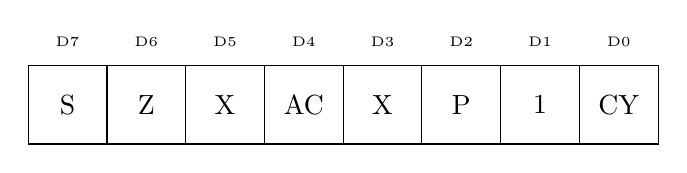
\begin{tikzpicture}
    \foreach \x/\label/\bit in {0/S/D7, 1/Z/D6, 2/X/D5, 3/AC/D4, 4/X/D3, 5/P/D2, 6/1/D1, 7/CY/D0} {
        \draw (\x,0) rectangle (\x+1,1);
        \node at (\x+0.5, 0.5) {\label};
        \node at (\x+0.5, 1.3) {\tiny \bit};
    }
\end{tikzpicture}
\end{center}

\begin{itemize}
    \item \textbf{S (Sign)}: Set if D7 is 1 (Negative result)
    \item \textbf{Z (Zero)}: Set if result is zero
    \item \textbf{AC (Auxiliary Carry)}: Carry from D3 to D4
    \item \textbf{P (Parity)}: Set if result has even number of 1s
    \item \textbf{CY (Carry)}: Carry out from D7
\end{itemize}
\end{solutionbox}
\begin{mnemonicbox}
``SuZie AC's Perfect CarrY''
\end{mnemonicbox}

\orquestionmarks{2}{c}{7}
\textbf{Describe Pin diagram of 8085 microprocessor with the help of neat diagram.}

\begin{solutionbox}
\textbf{Answer}:

\textbf{Pin Diagram:}
\begin{center}
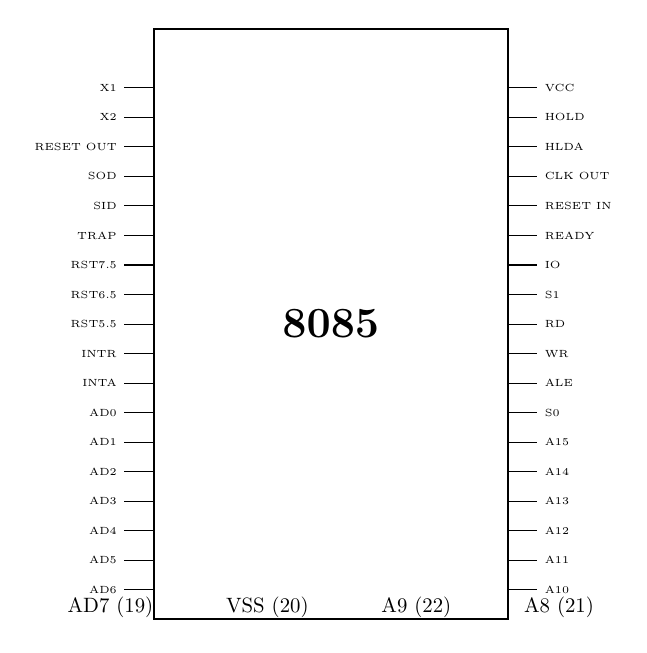
\begin{tikzpicture}[scale=0.75, transform shape]
    \draw [thick] (0,0) rectangle (6,10);
    \node at (3,5) {\huge \textbf{8085}};
    
    % Left Side
    \foreach \y/\lab in {9/X1, 8.5/X2, 8/RESET OUT, 7.5/SOD, 7/SID, 6.5/TRAP, 6/RST7.5, 5.5/RST6.5, 5/RST5.5, 4.5/INTR, 4/INTA, 3.5/AD0, 3/AD1, 2.5/AD2, 2/AD3, 1.5/AD4, 1/AD5, 0.5/AD6} {
        \draw (-0.5, \y) -- (0, \y); \node [left] at (-0.5, \y) {\tiny \lab};
    }
    
    % Right Side
    \foreach \y/\lab in {9/VCC, 8.5/HOLD, 8/HLDA, 7.5/CLK OUT, 7/RESET IN, 6.5/READY, 6/IO/M, 5.5/S1, 5/RD, 4.5/WR, 4/ALE, 3.5/S0, 3/A15, 2.5/A14, 2/A13, 1.5/A12, 1/A11, 0.5/A10} {
        \draw (6, \y) -- (6.5, \y); \node [right] at (6.5, \y) {\tiny \lab};
    }
    
    \node at (3, 0.2) {AD7 (19) \hspace{1cm} VSS (20) \hspace{1cm} A9 (22) \hspace{1cm} A8 (21)};
\end{tikzpicture}
\end{center}

\begin{itemize}
    \item \textbf{Address/Data}: Multiplexed AD0-AD7, A8-A15
    \item \textbf{Control}: RD, WR, IO/M, ALE
    \item \textbf{Interrupts}: TRAP, RST 7.5/6.5/5.5, INTR
    \item \textbf{Power}: VCC (+5V), VSS (GND)
\end{itemize}
\end{solutionbox}
\begin{mnemonicbox}
``ACID-PS: Address-Control-Interrupt-DMA-Power-Serial''
\end{mnemonicbox}

\questionmarks{3}{a}{3}
\textbf{Explain Stack, Stack Pointer and Stack operation.}

\begin{solutionbox}
\textbf{Answer}:

\begin{itemize}
    \item \textbf{Stack}: Reserved area of RAM used for temporary storage (LIFO).
    \item \textbf{Stack Pointer (SP)}: 16-bit register holding address of top of stack.
    \item \textbf{PUSH}: Decrement SP, Store data.
    \item \textbf{POP}: Retrieve data, Increment SP.
\end{itemize}

\textbf{Diagram:}
\begin{center}
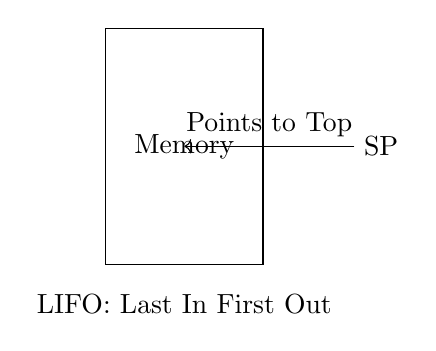
\begin{tikzpicture}[node distance=1.5cm, auto]
    \node [draw, minimum width=2cm, minimum height=3cm] (stack) {Memory};
    \node [right of=stack, node distance=2.5cm] (sp) {SP};
    \draw [->] (sp) -- (stack.center) node [midway, above] {Points to Top};
    
    \node [below of=stack, node distance=2cm] {LIFO: Last In First Out};
\end{tikzpicture}
\end{center}
\end{solutionbox}
\begin{mnemonicbox}
``SP Points to LIFO Lane''
\end{mnemonicbox}

\questionmarks{3}{b}{4}
\textbf{Draw Pin diagram of 8051 microcontroller.}

\begin{solutionbox}
\textbf{Answer}:

\begin{center}
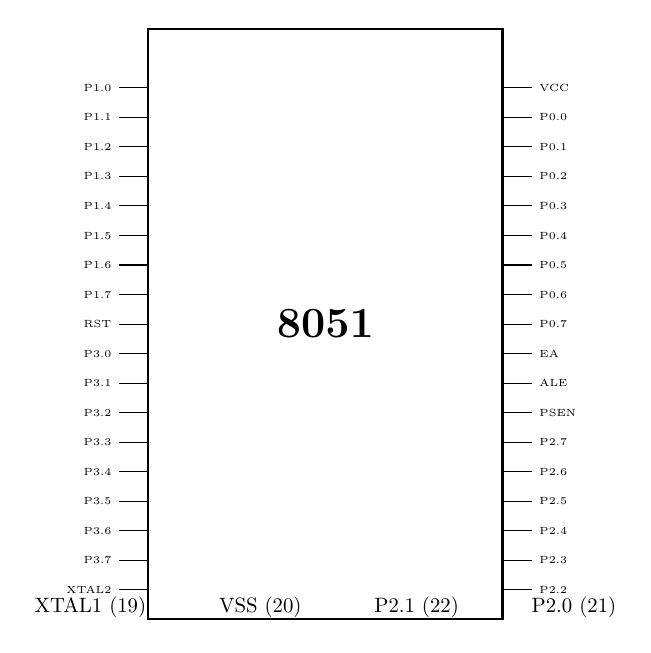
\begin{tikzpicture}[scale=0.75, transform shape]
    \draw [thick] (0,0) rectangle (6,10);
    \node at (3,5) {\huge \textbf{8051}};
    
    % Left Side (1-20)
    \foreach \y/\lab in {9/P1.0, 8.5/P1.1, 8/P1.2, 7.5/P1.3, 7/P1.4, 6.5/P1.5, 6/P1.6, 5.5/P1.7, 5/RST, 4.5/P3.0, 4/P3.1, 3.5/P3.2, 3/P3.3, 2.5/P3.4, 2/P3.5, 1.5/P3.6, 1/P3.7, 0.5/XTAL2} {
        \draw (-0.5, \y) -- (0, \y); \node [left] at (-0.5, \y) {\tiny \lab};
    }
    
    % Right Side (40-21)
    \foreach \y/\lab in {9/VCC, 8.5/P0.0, 8/P0.1, 7.5/P0.2, 7/P0.3, 6.5/P0.4, 6/P0.5, 5.5/P0.6, 5/P0.7, 4.5/EA, 4/ALE, 3.5/PSEN, 3/P2.7, 2.5/P2.6, 2/P2.5, 1.5/P2.4, 1/P2.3, 0.5/P2.2} {
        \draw (6, \y) -- (6.5, \y); \node [right] at (6.5, \y) {\tiny \lab};
    }
    
    \node at (3, 0.2) {XTAL1 (19) \hspace{1cm} VSS (20) \hspace{1cm} P2.1 (22) \hspace{1cm} P2.0 (21)};
\end{tikzpicture}
\end{center}

\begin{itemize}
    \item \textbf{P0}: Multiplexed Address/Data
    \item \textbf{P1}: General I/O
    \item \textbf{P2}: High Order Address
    \item \textbf{P3}: Special Functions (Serial, Int, Timer)
\end{itemize}
\end{solutionbox}
\begin{mnemonicbox}
``PORT 0123: Data-General-Address-Special''
\end{mnemonicbox}

\questionmarks{3}{c}{7}
\textbf{Draw Timers/Counters logic diagram of 8051 microcontroller and explain its operation in various modes.}

\begin{solutionbox}
\textbf{Answer}:

\textbf{Logic Diagram:}
\begin{center}
\begin{tikzpicture}[node distance=2.5cm, auto]
    \node [gtu block] (osc) {Oscillator\\$\div$ 12};
    \node [gtu block, right of=osc, node distance=3cm] (control) {Control\\(C/T, GATE)};
    \node [gtu block, right of=control, node distance=3cm] (tl) {TLx\\(8-bit)};
    \node [gtu block, right of=tl] (th) {THx\\(8-bit)};
    
    \draw [gtu arrow] (osc) -- (control);
    \draw [gtu arrow] (control) -- (tl);
    \draw [gtu arrow] (tl) -- (th);
    \draw [gtu arrow, ->] (th) -- ++(1,0) node[right] {Interrupt};
    
    \node [below of=control] (pin) {Pin (Tn)};
    \draw [gtu arrow] (pin) -- (control);
\end{tikzpicture}
\end{center}

\textbf{Modes:}
\begin{itemize}
    \item \textbf{Mode 0}: 13-bit timer mode.
    \item \textbf{Mode 1}: 16-bit timer mode.
    \item \textbf{Mode 2}: 8-bit auto-reload mode.
    \item \textbf{Mode 3}: Split timer mode.
\end{itemize}
\end{solutionbox}
\begin{mnemonicbox}
``MARC: Mode Auto-Reload Count''
\end{mnemonicbox}

\orquestionmarks{3}{a}{3}
\textbf{List Common features of Microcontrollers.}

\begin{solutionbox}
\textbf{Answer}:

\begin{center}
\captionof{table}{MCU Features}
\begin{tabulary}{\linewidth}{|l|J|}
\hline
\textbf{Feature} & \textbf{Purpose} \\ \hline
\textbf{CPU Core} & Process instructions \\ \hline
\textbf{Memory} & Store program (ROM) and data (RAM) \\ \hline
\textbf{I/O Ports} & Interface with external devices \\ \hline
\textbf{Timers} & Measure time intervals \\ \hline
\textbf{Interrupts} & Handle asynchronous events \\ \hline
\textbf{Serial Comm} & Transfer data with other devices \\ \hline
\end{tabulary}
\end{center}
\end{solutionbox}
\begin{mnemonicbox}
``CRITICS: CPU ROM I/O Timers Interrupts Comm Serial''
\end{mnemonicbox}

\orquestionmarks{3}{b}{4}
\textbf{Explain Internal RAM Organization of 8051 microcontroller.}

\begin{solutionbox}
\textbf{Answer}:

\begin{center}
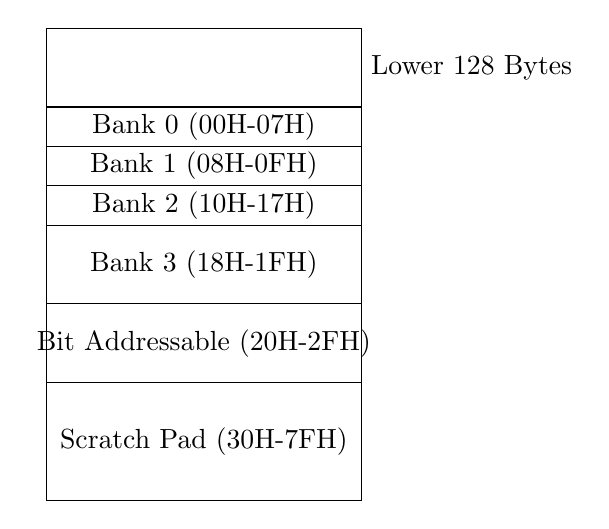
\begin{tikzpicture}
    % RAM Map
    \draw (0,0) rectangle (4,6);
    
    \draw (0,1.5) -- (4,1.5);
    \node at (2, 0.75) {Scratch Pad (30H-7FH)};
    
    \draw (0,2.5) -- (4,2.5);
    \node at (2, 2) {Bit Addressable (20H-2FH)};
    
    \draw (0,3.5) -- (4,3.5);
    \node at (2, 3) {Bank 3 (18H-1FH)};
    \draw (0,4) -- (4,4);
    \node at (2, 3.75) {Bank 2 (10H-17H)};
    \draw (0,4.5) -- (4,4.5);
    \node at (2, 4.25) {Bank 1 (08H-0FH)};
    \draw (0,5) -- (4,5);
    \node at (2, 4.75) {Bank 0 (00H-07H)};
    
    \node [right] at (4, 5.5) {Lower 128 Bytes};
\end{tikzpicture}
\end{center}

\begin{itemize}
    \item \textbf{Register Banks (00H-1FH)}: 4 banks of 8 registers (R0-R7).
    \item \textbf{Bit Addressable (20H-2FH)}: 16 bytes where each bit can be accessed.
    \item \textbf{Scratch Pad (30H-7FH)}: General purpose RAM.
    \item \textbf{SFRs (80H-FFH)}: Special Function Registers (upper 128 bytes).
\end{itemize}
\end{solutionbox}
\begin{mnemonicbox}
``RBBS: Registers Bits Buffer Scratch''
\end{mnemonicbox}

\orquestionmarks{3}{c}{7}
\textbf{Explain architecture of 8051 microcontroller with the help of neat diagram.}

\begin{solutionbox}
\textbf{Answer}:

\textbf{Diagram:}
\begin{center}
\begin{tikzpicture}[node distance=2.5cm, auto, scale=0.8, transform shape]
    \node [gtu block] (cpu) {CPU};
    \node [gtu block, left of=cpu, node distance=3.5cm] (rom) {4KB ROM};
    \node [gtu block, below of=rom] (ram) {128B RAM};
    \node [gtu block, right of=cpu, node distance=3.5cm] (int) {Interrupt\\Control};
    \node [gtu block, below of=int] (serial) {Serial Port};
    \node [gtu block, below of=cpu] (timer) {Timers\\T0, T1};
    \node [gtu block, below of=timer, node distance=2cm, minimum width=6cm] (ports) {I/O Ports P0-P3};
    
    \node [gtu block, above of=cpu] (osc) {Oscillator};
    \draw [gtu arrow] (osc) -- (cpu);
    
    \draw [gtu arrow, <->] (cpu) -- (rom);
    \draw [gtu arrow, <->] (cpu) -- (ram);
    \draw [gtu arrow, <->] (cpu) -- (ports);
\end{tikzpicture}
\end{center}

\begin{itemize}
    \item \textbf{CPU}: 8-bit central processor.
    \item \textbf{Memory}: 4KB ROM (Code), 128B RAM (Data).
    \item \textbf{I/O}: 4 Ports (P0-P3).
    \item \textbf{Timers}: 2 16-bit timers.
    \item \textbf{Serial}: 1 UART channel.
    \item \textbf{Interrupts}: 5 sources.
\end{itemize}
\end{solutionbox}
\begin{mnemonicbox}
``CAPITALS: CPU Architecture Ports I/O Timer ALU LS-Interface Serial''
\end{mnemonicbox}

\questionmarks{4}{a}{3}
\textbf{Write an 8051 Assembly Language Program to Copy the data from external RAM Location 0123h to TL0 and Data from external RAM location 0234h to TH0.}

\begin{solutionbox}
\textbf{Answer}:

\begin{lstlisting}[language=8051]
MOV  DPTR, #0123H   ; Load DPTR with source address 0123H
MOVX A, @DPTR       ; Read data from external RAM
MOV  TL0, A         ; Copy to Timer 0 low byte

MOV  DPTR, #0234H   ; Load DPTR with source address 0234H
MOVX A, @DPTR       ; Read data from external RAM
MOV  TH0, A         ; Copy to Timer 0 high byte
\end{lstlisting}
\end{solutionbox}
\begin{mnemonicbox}
``DRAM: DPTR Read Address Move''
\end{mnemonicbox}

\questionmarks{4}{b}{4}
\textbf{Write an 8051 Assembly Language Program to blink LED interfaced at port P1.3 at time interval of 1ms.}

\begin{solutionbox}
\textbf{Answer}:

\begin{lstlisting}[language=8051]
AGAIN:  SETB P1.3         ; Turn ON LED at P1.3
        ACALL DELAY       ; Call delay subroutine
        CLR  P1.3         ; Turn OFF LED at P1.3
        ACALL DELAY       ; Call delay subroutine
        SJMP AGAIN        ; Repeat forever

DELAY:  MOV  R7, #250     ; Load R7 for outer loop
OUTER:  MOV  R6, #1       ; Load R6 for inner loop
INNER:  DJNZ R6, INNER    ; Decrement R6 until zero
        DJNZ R7, OUTER    ; Decrement R7 until zero
        RET               ; Return from subroutine
\end{lstlisting}
\end{solutionbox}
\begin{mnemonicbox}
``STACI: Set-Timer-And-Clear-Infinitely''
\end{mnemonicbox}

\questionmarks{4}{c}{7}
\textbf{List Addressing Modes of 8051 Microcontroller and explain all of them with the help of example.}

\begin{solutionbox}
\textbf{Answer}:

\begin{center}
\captionof{table}{Addressing Modes}
\begin{tabulary}{\linewidth}{|l|l|J|}
\hline
\textbf{Addressing Mode} & \textbf{Example} & \textbf{Description} \\ \hline
\textbf{Immediate} & \code{MOV A, \#25H} & Data is in instruction \\ \hline
\textbf{Register} & \code{MOV A, R0} & Data is in register \\ \hline
\textbf{Direct} & \code{MOV A, 30H} & Data is at RAM address \\ \hline
\textbf{Indirect} & \code{MOV A, @R0} & R0/R1 contains address \\ \hline
\textbf{Indexed} & \code{MOVC A, @A+DPTR} & Access program memory \\ \hline
\textbf{Bit} & \code{SETB P1.3} & Access individual bits \\ \hline
\textbf{Relative} & \code{SJMP LABEL} & Jumps with 8-bit offset \\ \hline
\end{tabulary}
\end{center}
\end{solutionbox}
\begin{mnemonicbox}
``I'M DIRBI: Immediate Register Direct Bit Indexed''
\end{mnemonicbox}

\orquestionmarks{4}{a}{3}
\textbf{Write an 8051 Assembly Language Program to Subtract the content of RAM location 11h from RAM location 14h; put result in RAM location 3Ch.}

\begin{solutionbox}
\textbf{Answer}:

\begin{lstlisting}[language=8051]
MOV  A, 14H       ; Load content of RAM location 14H to A
CLR  C            ; Clear carry flag
SUBB A, 11H       ; Subtract content of 11H with borrow
MOV  3CH, A       ; Store result in RAM location 3CH
\end{lstlisting}
\end{solutionbox}
\begin{mnemonicbox}
``LCSS: Load-Clear-Subtract-Store''
\end{mnemonicbox}

\orquestionmarks{4}{b}{4}
\textbf{Write an 8051 Assembly Language Program to generate a square wave of 50\% duty cycle on bit 3 of Port 1 using Timer 0 in Mode 1.}

\begin{solutionbox}
\textbf{Answer}:

\begin{lstlisting}[language=8051]
      MOV  TMOD, #01H   ; Timer 0, Mode 1 (16-bit)
AGAIN: MOV  TH0, #0FCH   ; Load high byte
      MOV  TL0, #18H    ; Load low byte (-1000 in 16-bit)
      SETB TR0          ; Start timer
      JNB  TF0, $       ; Wait for overflow
      CLR  TR0          ; Stop timer
      CLR  TF0          ; Clear timer flag
      CPL  P1.3         ; Toggle P1.3
      SJMP AGAIN        ; Repeat
\end{lstlisting}
\end{solutionbox}
\begin{mnemonicbox}
``MSTCCS: Mode-Set-Timer-Check-Clear-Switch''
\end{mnemonicbox}

\orquestionmarks{4}{c}{7}
\textbf{Explain any seven Logical Instructions with example for 8051 Microcontroller.}

\begin{solutionbox}
\textbf{Answer}:

\begin{center}
\captionof{table}{Logical Instructions}
\begin{tabulary}{\linewidth}{|l|l|J|}
\hline
\textbf{Instruction} & \textbf{Example} & \textbf{Operation} \\ \hline
\textbf{ANL} & \code{ANL A, \#3FH} & Logical AND \\ \hline
\textbf{ORL} & \code{ORL P1, \#80H} & Logical OR \\ \hline
\textbf{XRL} & \code{XRL A, R0} & Logical XOR \\ \hline
\textbf{CLR} & \code{CLR A} & Clear (set to 0) \\ \hline
\textbf{CPL} & \code{CPL P1.0} & Complement (invert) \\ \hline
\textbf{RL} & \code{RL A} & Rotate left \\ \hline
\textbf{RR} & \code{RR A} & Rotate right \\ \hline
\end{tabulary}
\end{center}
\end{solutionbox}
\begin{mnemonicbox}
``A-OX-CCR: AND OR XOR Clear Complement Rotate''
\end{mnemonicbox}

\questionmarks{5}{a}{3}
\textbf{Draw Interfacing of Push button Switch with 8051 microcontroller.}

\begin{solutionbox}
\textbf{Answer}:

\textbf{Diagram:}
\begin{center}
\begin{tikzpicture}[node distance=2cm, auto]
    \node (vcc) {Vcc};
    \node [resistor, below of=vcc] (res) {10K};
    \node [below of=res] (junc) {};
    \node [left of=junc] (pin) {P1.0 (8051)};
    \node [push button, below of=junc] (btn) {Load};
    \node [ground, below of=btn] (gnd) {};
    
    \draw (vcc) -- (res) -- (junc);
    \draw (junc) -- (pin);
    \draw (junc) -- (btn) -- (gnd);
\end{tikzpicture}
\end{center}

\begin{itemize}
    \item \textbf{Pull-up Resistor}: Keeps pin HIGH when button is open.
    \item \textbf{Button Press}: Pulls pin LOW.
\end{itemize}
\end{solutionbox}
\begin{mnemonicbox}
``PIP: Pull-up-Input-Press''
\end{mnemonicbox}

\questionmarks{5}{b}{4}
\textbf{Interface Relay with 8051 microcontroller.}

\begin{solutionbox}
\textbf{Answer}:

\textbf{Diagram:}
\begin{center}
\begin{tikzpicture}[node distance=2.5cm, auto]
    \node (pin) {P1.0};
    \node [resistor, right of=pin] (base_res) {330$\Omega$};
    \node [npn, right of=base_res, anchor=B] (trans) {BC547};
    \node [ground, below of=trans] (gnd) {};
    
    \draw (pin) -- (base_res) -- (trans.B);
    \draw (trans.E) -- (gnd);
    
    % Relay Coil
    \node [coordinate, above of=trans, node distance=2cm] (coil_bottom) {};
    \draw (trans.C) -- (coil_bottom);
    \draw [inductor] (coil_bottom) -- ++(0,2) node[above] (vcc) {+5V};
    
    % Diode
    \draw (coil_bottom) -- ++(1,0) coordinate (d_bot);
    \draw (vcc|-d_bot) -- ++(1,0) coordinate (d_top);
    \draw [diode] (d_bot) -- (d_top);
    
    % Relay Switch
    \draw (d_top) -- ++(1.5,0) node[right] {Relay Common};
    \draw (d_top) ++(1.5,-1) node[right] {NO Contact} -- ++(0.5,0) node[right] {Load};
    
\end{tikzpicture}
\end{center}
\end{solutionbox}
\begin{mnemonicbox}
``TRIP: Transistor-Relay-Interface-Protection''
\end{mnemonicbox}

\questionmarks{5}{c}{7}
\textbf{Interface ADC0804 with 8051 microcontroller.}

\begin{solutionbox}
\textbf{Answer}:

\textbf{Diagram:}
\begin{center}
\begin{tikzpicture}[node distance=3cm, auto]
    \node [gtu block, minimum width=3cm, minimum height=4cm] (adc) {ADC0804};
    \node [gtu block, right of=adc, node distance=5cm, minimum width=3cm, minimum height=4cm] (mcu) {8051};
    
    \draw [gtu arrow, <->] (adc.10) -- (mcu.170) node[midway, above] {Data Bus (D0-D7)};
    
    \draw [gtu arrow, <-] (adc.-10) -- (mcu.-170) node[midway, below] {CS (P3.0)};
    \draw [gtu arrow, <-] (adc.-30) -- (mcu.-150) node[midway, below] {RD (P3.1)};
    \draw [gtu arrow, <-] (adc.-50) -- (mcu.-130) node[midway, below] {WR (P3.2)};
    \draw [gtu arrow, ->] (adc.-70) -- (mcu.-110) node[midway, below] {INTR (P3.3)};
    
    \node [left of=adc] (vin) {Analog In};
    \draw [gtu arrow] (vin) -- (adc);
\end{tikzpicture}
\end{center}

\begin{itemize}
    \item \textbf{Data Bus}: P1.0-P1.7 connected to D0-D7.
    \item \textbf{Control}: RD, WR, INTR for handshaking.
\end{itemize}
\end{solutionbox}
\begin{mnemonicbox}
``CRIW: Control-Read-Interrupt-Write''
\end{mnemonicbox}

\orquestionmarks{5}{a}{3}
\textbf{List Applications of microcontroller in various fields.}

\begin{solutionbox}
\textbf{Answer}:

\begin{center}
\captionof{table}{Applications}
\begin{tabulary}{\linewidth}{|l|J|}
\hline
\textbf{Field} & \textbf{Applications} \\ \hline
\textbf{Industrial} & Motor control, automation, PLCs \\ \hline
\textbf{Medical} & Patient monitoring, diagnostic equipment \\ \hline
\textbf{Consumer} & Washing machines, microwaves, toys \\ \hline
\textbf{Automotive} & Engine control, ABS, airbag systems \\ \hline
\textbf{Communication} & Mobile phones, modems, routers \\ \hline
\textbf{Security} & Access control, alarm systems \\ \hline
\end{tabulary}
\end{center}
\end{solutionbox}
\begin{mnemonicbox}
``I-MACS: Industrial-Medical-Automotive-Consumer-Security''
\end{mnemonicbox}

\orquestionmarks{5}{b}{4}
\textbf{Interface Stepper motor with 8051 microcontroller.}

\begin{solutionbox}
\textbf{Answer}:

\textbf{Diagram:}
\begin{center}
\begin{tikzpicture}[node distance=2.5cm, auto]
    \node [gtu block] (mcu) {8051\\(P1.0-P1.3)};
    \node [gtu block, right of=mcu, node distance=3.5cm] (driver) {ULN2003\\Driver};
    \node [gtu block, right of=driver, node distance=3.5cm] (motor) {Stepper\\Motor};
    
    \draw [gtu arrow, ->] (mcu) -- (driver) node[midway, above] {Control};
    \draw [gtu arrow, ->] (driver) -- (motor) node[midway, above] {High Current};
    
    \node [above of=driver, node distance=1.5cm] (vcc) {+12V};
    \draw [->] (vcc) -- (driver);
\end{tikzpicture}
\end{center}

\textbf{Sequence (Clockwise):} 0x08, 0x0C, 0x04, 0x06.
\end{solutionbox}
\begin{mnemonicbox}
``PDCS: Port-Driver-Current-Sequence''
\end{mnemonicbox}

\orquestionmarks{5}{c}{7}
\textbf{Interface LCD with 8051 microcontroller.}

\begin{solutionbox}
\textbf{Answer}:

\textbf{Diagram:}
\begin{center}
\begin{tikzpicture}[node distance=3cm, auto]
    \node [gtu block, minimum width=3cm, minimum height=4cm] (mcu) {8051};
    \node [gtu block, right of=mcu, node distance=5cm, minimum width=3cm, minimum height=3cm] (lcd) {16x2 LCD};
    
    \draw [gtu arrow, ->] (mcu.10) -- (lcd.170) node[midway, above] {Data (P2)};
    
    \draw [gtu arrow, ->] (mcu.-10) -- (lcd.-170) node[midway, below] {RS (P3.0)};
    \draw [gtu arrow, ->] (mcu.-30) -- (lcd.-150) node[midway, below] {RW (P3.1)};
    \draw [gtu arrow, ->] (mcu.-50) -- (lcd.-130) node[midway, below] {E (P3.2)};
\end{tikzpicture}
\end{center}

\begin{itemize}
    \item \textbf{Data}: Port 2 sends ASCII data/commands.
    \item \textbf{RS}: 0 for Command, 1 for Data.
    \item \textbf{E}: Enable Pulse to latch data.
\end{itemize}
\end{solutionbox}
\begin{mnemonicbox}
``DICE: Data-Instruction-Control-Enable''
\end{mnemonicbox}

\end{document}
